
%(BEGIN_QUESTION)
% Copyright 2009, Tony R. Kuphaldt, released under the Creative Commons Attribution License (v 1.0)
% This means you may do almost anything with this work of mine, so long as you give me proper credit

Read and outline the ``4-Way Solenoid Valves'' subsection of the ``Solenoid valves'' section of the ``Discrete Control Elements'' chapter in your {\it Lessons In Industrial Instrumentation} textbook.  Note the page numbers where important illustrations, photographs, equations, tables, and other relevant details are found.  Prepare to thoughtfully discuss with your instructor and classmates the concepts and examples explored in this reading.

\underbar{file i04195}
%(END_QUESTION)




%(BEGIN_ANSWER)


%(END_ANSWER)





%(BEGIN_NOTES)

4-way valves are used to reverse the direction of fluid flow to/from some kind of actuating mechanism such as a cylinder or a fluid motor.  

$$\includegraphics[width=15.5cm]{i04195x01.eps}$$

Spool-valve construction is typical for 4-way solenoid valves, due to the inherent {\it pressure-balanced} construction of this design which reduces the necessary force to actuate the spool.

$$\includegraphics[width=15.5cm]{i04195x02.eps}$$







\vskip 20pt \vbox{\hrule \hbox{\strut \vrule{} {\bf Suggestions for Socratic discussion} \vrule} \hrule}

\begin{itemize}
\item{} {\bf Present a 4-way solenoid valve to students for their inspection, challenging them to identify all ports on the valve.  If practical, set up a power supply to energize the solenoid so they may test its operation by blowing air through the ports in different energization states.}
\item{} Explain how to interpret ``box'' symbols for solenoid valves.
\item{} Explain how to interpret P\&ID symbols for solenoid valves.
\item{} Explain how spool valves are {\it pressure-balanced} to cancel all hydrostatic forces on the spool for easy actuation, referring to their cut-away diagrams for reference.
\item{} Locate one of the cut-away pictorial diagrams of a 4-way spool valve shown in the textbook and explain its operation.
\item{} Examining the three different styles of 4-way spool valves shown in cut-away view, identify which one will allow the final control element to ``drift'' in position when the spool is in the ``neutral'' (middle) position.
\item{} Locate the photograph of a Parker fluid power valve (in the textbook) and draw its valve symbol on a piece of paper, explaining the operation of that valve in as much detail as possible based on information contained in the photograph.
\end{itemize}


%INDEX% Reading assignment: Lessons In Industrial Instrumentation, Solenoid Valves (4-way solenoid valves and symbols)

%(END_NOTES)


